%%% Local Variables:
%%% mode: latex
%%% TeX-master: t
%%% End:

\documentclass{article}

\usepackage{fullpage}
\usepackage[utf8]{inputenc}
\usepackage{listings}
\usepackage[table]{xcolor}
\usepackage{amssymb}
\usepackage{amsmath}
\usepackage{fancyhdr}
\usepackage{lastpage}
\usepackage{parskip}
\usepackage{abstract}
\usepackage{url}
\usepackage{float}
\usepackage{enumitem}
\usepackage{fancybox}
\usepackage{amsmath}
\usepackage{graphicx}
\usepackage[bottom]{footmisc}
\usepackage{hyperref}
\usepackage{makecell}
\usepackage{tikz}
\usetikzlibrary{arrows,automata}


% constants
\newcommand{\COURSE}{02257 Applied Functional Programming}
\newcommand{\TITLE}{Project 3}
\newcommand{\DATE}{January 20, 2015}


%%% Local Variables:
%%% mode: latex
%%% TeX-master: "report"
%%% End:
\newcommand{\code}[1]{\texttt{#1}}
\newcommand{\fn}[2]{\lambda{} \ #1 \mapsto{} #2 }
\newcommand{\ite}[3]{\texttt{ if } #1 \texttt{ then } #2 \texttt{ else } #3 }
\newcommand{\qcol}{\quad:\quad}
\newcommand{\qvd}{\quad\vdash\quad}
%% source / reference
\newcommand{\refgeneral}[3]{#1 (#3), \emph{#2}}
% arguments:
% author
% title
% year
% publisher
\newcommand{\refbook}[4]{\refgeneral{#1}{#2}{#3}, #4}
% arguments:
% author
% title
% year
% url
\newcommand{\refonline}[4]{\refgeneral{#1}{#2}{#3} \\\url{<#4>}}
\definecolor{Brown}{cmyk}{0,0.81,1,0.60}
\definecolor{OliveGreen}{cmyk}{0.64,0,0.95,0.40}
\definecolor{CadetBlue}{cmyk}{0.62,0.57,0.23,0}
\definecolor{lightlightgray}{gray}{0.95}
\definecolor{lightgray}{gray}{0.85}
\definecolor{sh_comment}{rgb}{0.12, 0.38, 0.18}
\definecolor{sh_keyword}{rgb}{0.37, 0.38, 0.75}
\definecolor{sh_string}{rgb}{0.06, 0.10, 0.98}
\lstset{
basicstyle=\small\ttfamily,
stringstyle=\color{sh_string},
keywordstyle = \color{sh_keyword}\bfseries,
commentstyle=\color{sh_comment},
backgroundcolor=\color{lightlightgray},
frame=single,
rulecolor=\color{lightgray},
framesep=3pt,
numbersep=5pt,
xleftmargin=10pt,
xrightmargin=10pt,
showspaces=false,
showstringspaces=false,
tabsize=4,
aboveskip=5pt,
belowskip=5pt,
lineskip=2pt,
captionpos=b,
numbers=left,
numberstyle=\tiny,
stepnumber=1,
numbersep=100pt,
breaklines,
numbersep=5pt,
breakatwhitespace=false,
showspaces=false,
showtabs=false
}
\lstdefinelanguage{llvm}{
morecomment = [l]{;},
morestring=[b]",
sensitive = true,
classoffset=0,
morekeywords={
define, declare, global, constant,
internal, external, private,
linkonce, linkonce_odr, weak, weak_odr, appending,
common, extern_weak,
thread_local, dllimport, dllexport,
hidden, protected, default,
except, deplibs,
volatile, fastcc, coldcc, cc, ccc,
x86_stdcallcc, x86_fastcallcc,
ptx_kernel, ptx_device,
signext, zeroext, inreg, sret, nounwind, noreturn,
nocapture, byval, nest, readnone, readonly, noalias, uwtable,
inlinehint, noinline, alwaysinline, optsize, ssp, sspreq,
noredzone, noimplicitfloat, naked, alignstack,
module, asm, align, tail, to,
addrspace, section, alias, sideeffect, c, gc,
target, datalayout, triple,
blockaddress
},
classoffset=1, keywordstyle=\color{purple},
morekeywords={
fadd, sub, fsub, mul, fmul,
sdiv, udiv, fdiv, srem, urem, frem,
and, or, xor,
icmp, fcmp,
eq, ne, ugt, uge, ult, ule, sgt, sge, slt, sle,
oeq, ogt, oge, olt, ole, one, ord, ueq, ugt, uge,
ult, ule, une, uno,
nuw, nsw, exact, inbounds,
phi, call, select, shl, lshr, ashr, va_arg,
trunc, zext, sext,
fptrunc, fpext, fptoui, fptosi, uitofp, sitofp,
ptrtoint, inttoptr, bitcast,
ret, br, indirectbr, switch, invoke, unwind, unreachable,
malloc, alloca, free, load, store, getelementptr,
extractelement, insertelement, shufflevector,
extractvalue, insertvalue,
},
alsoletter={\%},
keywordsprefix={\%},
}
\lstdefinelanguage{JavaScript}{
keywords={typeof, new, true, false, catch, function, return, null, catch, switch, var, if, in, while, do, else, case, break},
keywordstyle=\color{blue}\bfseries,
ndkeywords={class, export, boolean, throw, implements, import, this},
ndkeywordstyle=\color{darkgray}\bfseries,
identifierstyle=\color{black},
sensitive=false,
comment=[l]{//},
morecomment=[s]{/*}{*/},
commentstyle=\color{purple}\ttfamily,
stringstyle=\color{red}\ttfamily,
morestring=[b]',
morestring=[b]"
}
\makeatother



\lstnewenvironment{promela}[0]{
\lstset{language=C++,
,morekeywords={if, then, else, return, function, var, for, foreach, do, end, od, fi}}
}
{}

\lstnewenvironment{java}[0]{
\lstset{language=C++,
}}
{}

% pseudo code environment
\lstnewenvironment{pseudo}[0]{
\lstset{
language=java
}}
{}


\pagestyle{fancy}
\fancyhf{}
\setlength{\parindent}{0pt}
\setlength{\headheight}{15pt}
\setlength{\headsep}{25pt}
\lhead{\COURSE}
\chead{\TITLE}
\rhead{\DATE}
\cfoot{Page \thepage{} of~\pageref{LastPage}}


\title{\TITLE\\ {\large \COURSE}}
\date{\DATE}
\author{
  Markus Færevaag {\tt s123692}\\
  Simon Altschuler {\tt s123563}
}


\begin{document}
\maketitle
\vspace{10cm}
\doublesignature{Markus Færevaag}{Simon Altschuler} \\
\clearpage

\section{Introduction}
In this report we will describe our experience with implementing the game Nim in F\# using asynchronuos computations.

A note on Nim rules; there are two variations of the game namely mis\`ere and normal play. We have implemented normal play meaning that the winner is the one who takes the last match.

\section{Status}
The game implements all required as well as optional features. The \texttt{Nim.Driver} modules, which manages the flow of application control, utilizes F\#'s \texttt{async} capabilities along with Don Syme's \texttt{AsyncEventQueue}.

The game can fetch games from URLs in the given format, namely a sorted list of heap sizes separated by space.

It is possible to play against the computer, which will punish even the slightest inaccurate move with certain victory. It does this by following a set of fairly simple rules.

We have designed the program in a modular way have achieved a good separation of concerns. To demonstrate that, we have implemented two different user interfaces; a GUI and a CLI. The compiled executable can be run with the command line argument \texttt{-nw} to use the CLI.

The GUI is somewhat pleasing to use, and allows the user to remove matches by clicking on the desired row at the number of matches to remove.

A taunt messages appears when the user slips and lets the computer take the advantage and permanently establish the coming victory.

\section{Computer player}
To implement the AI one must compute the so-called nim sum of the board. This is a simple matter of XOR'ing all heaps on the board.

The computer only knows two states of the game:
\begin{description}
\item[Nim sum is $0$:] This is the loosing state and the AI will just remove a single match from the largest heap and hope for the user to blunder.

\item[Nim sum is not $0$:] This is the winning state and to stay in the lead we must find a move that yields a state with a nim sum of $0$. This is done by identifying a heap which decreases when XOR'ed with the nim sum. The optimal move is then to reduce that heap's size by the computed nim sum.
\end{description}

\section{Modular design}
We have designed the program in a way that enforces strict separation of concerns. Following is a brief description of each module and its responsibility:


\begin{description}
\item[Main] Bootstraps the
\item[Core] Handles game logic of Nim, defines types \texttt{Heap}, \texttt{Board} and \texttt{Game} that expose functions such as \texttt{Move} and \texttt{ComputerMove}
\item[Driver] Handles the flow of the program (see \ref{sec:fsa})
\item[Exceptions] Implements some exceptions that can be thrown, for instance \texttt{InvalidMove} and \texttt{ParseError}
\item[GUI] Defines the \texttt{GUI} variant of the game
\item[CLI] Defines the \texttt{CLI} variant of the game in which the user can type commands into a REPL-like environment
\item[Service] The module that is responsible for fetching content from a URL
\item[UI] Defines the interface that user interfaces must adhere to. Also defines the different states that a UI must be able to render (\texttt{UIState})
\item[Utils] Some helper functions for lists and the parser of downloaded nim games
\end{description}

\section{User Interfaces}
To demonstrate the modularity of this solution we have chosen to implement two different user interfaces, each implementing the {\tt UI} interface. We have made a graphical user interface (GUI) which uses {\tt Windows.Forms}, called {\tt GUI}, and a command-line interface with a read-eval-print loop (REPL), called {\tt CLI}.

The {\tt Driver}, which contains the flow logic of the program, is given a user interface implementing the {\tt UI} interface, so the interface logic is completely encapsulated in the respective interface implementations.

The user interface is chosen run-time by passing the program a command line argument. Given then {\tt -nw} (no-window) argument, it uses the command-line interface, while the graphical interface is chosen by default.

\section{Finite-State Automata}
The finitie-state automata that describes the interactions possible when playing the game.
\label{sec:fsa}
\begin{figure}[H]
\begin{tikzpicture}[auto, thick, node distance=3.6cm, yscale=2.0]

  \node[initial,state, minimum size=2cm] (ready)                            {{\tt ready}};
  \node[state, minimum size=2cm]         (loading)    [right of=ready]      {{\tt loading}};
  \node[state, minimum size=2cm]         (cancelling) [right of=loading]    {{\tt cancelling}};
  \node[state, minimum size=2cm]         (play)       [right of=cancelling] {{\tt play}};
  \node[state, minimum size=2cm]         (finished)   [right of=play]       {{\tt finished}};

  \path[->] (ready) edge [loop above, yscale=0.5] node {{\tt *}}        (ready)
                    edge                          node {{\tt Load}}     (loading)
          (loading) edge                          node {{\tt Cancel}}   (cancelling)
                    edge [bend left, below]       node {{\tt Loaded}}   (play)
                    edge [bend left, pos=0.2]     node {{\tt Error, *}} (ready)
       (cancelling) edge [bend left, pos=0.2]     node {{\tt *}}        (ready)
             (play) edge [loop above, yscale=0.5] node {{\tt *}}        (play)
                    edge [bend left, pos=0.2]     node {{\tt Cancel}}   (ready)
                    edge                          node {{\tt Finished}} (finished)
         (finished) edge [bend right, above]      node {{\tt Load}}     (loading)
                    edge [bend left, pos=0.2]     node {{\tt *}}        (ready);

\end{tikzpicture}

\caption{Finite-State Automata}
\end{figure}
\end{document}
